% !TEX TS-program = pdflatex
% !TEX encoding = UTF-8 Unicode

% This is a simple template for a LaTeX document using the "article" class.
% See "book", "report", "letter" for other types ofgit document.

\documentclass[12pt]{article} % use larger type; default would be 10pt
\usepackage[utf8]{inputenc}   % set input encoding (not needed with XeLaTeX)

%%% PAGE DIMENSIONS
\usepackage{geometry}
\geometry{a4paper}
\geometry{margin=1in} % 1in page margin

%%% COLOR AND GRAPHICS
\usepackage{color}
\usepackage{graphicx} % support the \includegraphics command and options
%\usepackage{caption}
%\usepackage{subcaption}

\usepackage{pslatex}
\definecolor{mygreen}{rgb}{0,0.6,0}
\definecolor{mygray}{rgb}{0.5,0.5,0.5}
\definecolor{mymauve}{rgb}{0.58,0,0.82}
\usepackage{listings} % For displaying source code
\lstset{ %
  language=C,                      % the language of the code
  backgroundcolor=\color{white},   % choose the background color; you must add \usepackage{color} or \usepackage{xcolor}
  basicstyle=\sffamily\fontsize{11}{13.2}\selectfont,        % the size of the fonts that are used for the code
  breakatwhitespace=false,         % sets if automatic breaks should only happen at whitespace
  breaklines=true,                 % sets automatic line breaking
  captionpos=t,                    % sets the caption-position to bottom
  commentstyle=\color{mygreen},    % comment style
  deletekeywords={...},            % if you want to delete keywords from the given language
  escapeinside={\%*}{*)},          % if you want to add LaTeX within your code
  extendedchars=true,              % lets you use non-ASCII characters; for 8-bits encodings only, does not work with UTF-8
  frame=single,                    % adds a frame around the code
  keepspaces=true,                 % keeps spaces in text, useful for keeping indentation of code (possibly needs columns=flexible)
  keywordstyle=\color{blue},       % keyword style
  morekeywords={*,...},            % if you want to add more keywords to the set
  numbers=left,                    % where to put the line-numbers; possible values are (none, left, right)
  numbersep=5pt,                   % how far the line-numbers are from the code
  numberstyle=\color{mygray},      % the style that is used for the line-numbers
  rulecolor=\color{black},         % if not set, the frame-color may be changed on line-breaks within not-black text (e.g. comments (green here))
  showspaces=false,                % show spaces everywhere adding particular underscores; it overrides 'showstringspaces'
  showstringspaces=false,          % underline spaces within strings only
  showtabs=false,                  % show tabs within strings adding particular underscores
  stepnumber=1,                    % the step between two line-numbers. If it's 1, each line will be numbered
  stringstyle=\color{mymauve},     % string literal style
  tabsize=2,                       % sets default tabsize to 2 spaces
  title=\lstname                   % show the filename of files included with \lstinputlisting; also try caption instead of title
}

% \usepackage[parfill]{parskip} % Activate to begin paragraphs with an empty line rather than an indent

%%% PACKAGES
\usepackage{booktabs} % for much better looking tables
\usepackage{array}    % for better arrays (eg matrices) in maths
\usepackage{paralist} % very flexible & customisable lists (eg. enumerate/itemize, etc.)
\usepackage{verbatim} % adds environment for commenting out blocks of text & for better verbatim
\usepackage{subfigure}

%%% HEADERS & FOOTERS
%\usepackage{fancyhdr} % This should be set AFTER setting up the page geometry
%\pagestyle{fancy} % options: empty , plain , fancy
%\renewcommand{\headrulewidth}{0pt} % customise the layout...
%\lhead{}\chead{}\rhead{}
%\lfoot{}\cfoot{\thepage}\rfoot{}


%%% SECTION TITLE APPEARANCE
\usepackage{sectsty}
\sectionfont{\normalsize\bfseries\uppercase}
\subsectionfont{\normalsize\bfseries}
\subsubsectionfont{\normalsize\mdseries\itshape}

%%% ToC (table of contents) APPEARANCE
\usepackage[nottoc,notlof,notlot]{tocbibind} % Put the bibliography in the ToC
\usepackage[titles,subfigure]{tocloft} % Alter the style of the Table of Contents
\renewcommand{\cftsecfont}{\rmfamily\mdseries\upshape}
\renewcommand{\cftsecpagefont}{\rmfamily\mdseries\upshape} % No bold!

%%% Title setup
\newcommand{\TitleFont}{\fontsize{16}{20}\selectfont\bfseries}
\newcommand{\AuthorFont}{\fontsize{14}{17}\selectfont}

%%% END Article customizations

%%% The "real" document content comes below...

\title{\TitleFont EE 472 Lab 3 \\ Learning the Development Environment - The Next Step \vfill }
\author{\AuthorFont Jonathan Ellington \\ Patrick Ma \\ Jarrett Gaddy}
\date{}

\begin{document}

%% Make title and ToC, start page numbering AFTER ToC
\maketitle
\thispagestyle{empty}
\pagebreak
\tableofcontents
\listoftables
\listoffigures
\thispagestyle{empty}
\pagebreak
\setcounter{page}{1}


\section{Abstract} In this lab the students are to take on the role of an
embedded system design team. They will design modifications to the medical
instrument previously designed. When the device finds metrics
are out of the acceptable range, the user is notified, thus saving them
from potential health risks. The students first laid out the design for
their system using various design tools, then they implemented the system in
software. Finally the students tested their system and verified that it is
ready to start saving lives. 

\section{Introduction}
The students are to design an embedded system on the Texas Instruments
Stellaris EKI-LM3S8962 and EE 472 embedded design testboard. The design must
implement a medical monitoring device. This device must monitor a patient's
temperature, heart rate, and blood pressure, as well as its own battery state.
The design must indicate when a monitored value is outside of a specified range
by flashing an LED on the test board. When a value deviates even further from
the valid range an alarm will sound. This alarm will sound until the values
return to the valid range or the user acknowledges the alarm with a button. The
values of each measurement will also be printed to the oled screen. This implementation will build upon the previous implementation of the device by adding functionality. Added functions include heart rate sensor, keypad input, menu display, data logging, and UART serial communication.

The design will be tested to verify proper behavior on alarm and warning notifications. In addition the implementation will be tested by measuring the amount of time that each of the 8 program tasks running the instrument take to execute. These tasks are mini programs that each handle a part of the instruments purpose.

\section{Discussion of the Lab}

\subsection{Design Specification\label{sec:designSpec}} 

\subsubsection{Specification Overview}
The entire system must satisfy several lofty objectives. The final product must
be portable, lightweight, and Internet-enabled. The system must also make
measurements of vital bodily functions, perform simple computations, provide
data logging functionality, and indicate when measured vitals exceed given
ranges, or the user fails to comply with a prescribed logging regimen. \\

\begin{itemize}[$$]
  \item The initial Phase 1 functional requirements for the system are:
    \begin{itemize}[$\bullet$]
      \item Provide continuous sensor monitoring capability
      \item Produce a visual display of the sensor values
      \item Accept variety of input data types
      \item Provide visual indication of warning states
      \item Provide an audible indicator of alarm states
    \end{itemize}
  \item In addition, the following requirements have been added:
    \begin{itemize}[$\bullet$]
      \item Utilize a hardware-based time reference
      \item support dynamic task creation and deletion
      \item support a user input device
      \item support data logging capabilities
      \item support remote communication capability
      \item Improve overall system performace
      \item Improve overall system safety
    \end{itemize}
\end{itemize}

\subsubsection{Identified Use Cases}
Taking the functional requirements listed above, several use cases were
developed. A Use case diagram of these scenarios is given in
Figure~\ref{fig:useCases}. Each use case is expanded and explained below.

\begin{figure}[h]
  \centering
  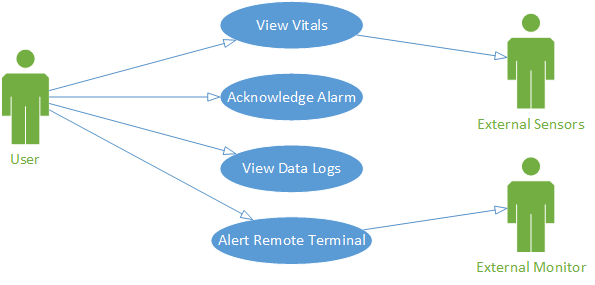
\includegraphics[width=\textwidth]{../design/use_cases_graphical.png}
  \caption{Use case diagram}
  \label{fig:useCases}
\end{figure}

~\\
\textbf{Use Case \#1: View Vital Measurements } \\
In the first use case, the user views the basic measurements picked up by the
sensors connected to the device. \\
During normal operation, once the device is turned on by the user, the system
records the value output by each sensor. This raw value is linearized and 
converted into a human-readable form. The user can select toggle between a
summary of current vitals as measured by the system or view measurements of
each sensor individually.

Three exceptional conditions were identified for this use case: 
\begin{itemize}
  \item \emph{One or more of the expected sensors is not connected} - If this occurs, the measurements taken by the device may be erratic. At the present moment, no action will be taken in such events. Later revisions may address the issue
  \item \emph{A measured value is outside 5\% of the specified normal range} - In this case, a warning signal will flash as an indication of the warning condition
  \item \emph{A measured value falls outside 10\% of a specified "normal" range} - In this case, an audible alarm will sound to indicate the alarm condition
\end{itemize}

~\\
\textbf{Use Case \#2: Acknowledge Alarm} \\
In the second case, the system is in an alarm state. The user acknowledges
the alarm condition by pressing a button.

Upon pressing the button, the system silences the audible alarm. Any visual
warnings continue to flash during the silenced period. If a significant amounts
of time pass and the sensor reading(s) continue to maintain an alarmed state,
the audible alarm will recommence.

No exceptional conditions were identified for this use case.\\

\textbf{Use Case \#3: View Measurement Logs} \\
In the third use case, the user wishes to view previously recorded measurements for a given vital sign.

As the device is running, the user opts to enter View Logs mode. From this
point, the user can select which vital sign they wish to examine. Upon
selection, the data logged from previous measurements is displayed.

Possible exception conditions may include the following:
\begin{itemize}
  \item \emph{User wishes to view more data than the machine remembers} - The
    machine will not support this operation. The system is only able to display
    the amount of data defined by the device. Future variants may support an
    external storage or logging functionality
  \item \emph{Machine loses power while reading or writing} - if the system
    loses power, any data stored in dynamic memory will be lost. On restart,
    data will be overwritten and lost. Future device versions may allow for
    storage in nonvolatile memory
  \item \emph{Ongoing measurements trigger warning or alarms} - since
    measurements are taken continuously, the device may enter an alarm or
    warning state. In this case, the display will not change unless prompted to
    by the user. Any alert indicators (visual, audible, or remote messaging)
    will operate as normal in the background
\end{itemize}

\textbf{Use Case \#4: System Alert to Remote Terminal}\\
In the event that the system enters an alert state (e.g. alarm or warning), the
system can send a message to a remote terminal connected to the device. The
messages sent can inform a second actor of the cause of alert and provide any
additional useful information.

Possible exception conditions may include:
\begin{itemize}
  \item \emph{Improper configuration of the Remote Terminal} - If the remote
    terminal connection is improperly configured or initialized, data received
    may be corrupted and not display properly. The device cannot ensure a
    proper connection and it is the responsibility of the remote user to ensure
    the correct configuration is used
  \item \emph{Remote Connection Lost} – If the user terminates the connection
    or the connection is lost, messages sent by the device may not arrive at
    the remote terminal or data may be corrupted. The device will not
    necessarily monitor the status of any remote connection; this
    responsibility is the remote terminals. In the event a connection is
    broken, the device system must continue to perform the other system
    functions without ill effects.
\end{itemize}


\subsubsection{Detailed Specifications (update)}
For this project, the requirements have been further specified as follows:

\begin{itemize}[$$]
  \item The system must have the following inputs:
    \begin{itemize}[$\bullet$]
      \item Alarm acknowledgment capability using a pushbutton
      \item Buttons or switches to allow user to access system modes and menu items
      \item Sensor measurement input capability consisting of:
	\begin{itemize}
	  \item Body temperature measurement
	  \item Pulse rate measurement signal
	  \item Systolic blood pressure measurement
	  \item Diastolic blood pressure measurement
	\end{itemize}
    \end{itemize}
\end{itemize}


\begin{itemize}[$$]
  \item The system must have the following outputs:
    \begin{itemize}[$\bullet$]
      \item Visual display of the following data in human-readable formats:
	\begin{itemize}
	  \item Body temperature
	  \item Pulse rate
	  \item Systolic blood pressure
	  \item Diastolic blood pressure
	  \item Battery status
	\end{itemize}
      \item Visually indicate warning state with a flashing LED
      \item Visually indicate a low battery state with an LED
      \item Audibly indicate an alarm state using a speaker
      \item External data connection to a remote terminal
    \end{itemize}
\end{itemize}

The initialization values, normal measurement ranges, displayed units, and 
warning and alarm behaviors for each vital measurement are given in 
Table~\ref{tab:sensorDefs}. The sensors must be sampled every five seconds and the system cannot block and cease operation for five seconds.

\begin{table}[h]
  \centering
  \begin{tabular}{|l|*{5}{c}|}
    \hline
    Measurement & Units & Initial Value & Min. Value & Max. Value & Warning Flash Period \\ \hline
    Body Temperature & C & 75 & 36.1C & 37.8C & 1 sec \\ \hline
    Systolic BP & mm Hg & 80 & - & 120 mmHg & 0.5 sec \\ \hline
    Diastolic BP & mm Hg & 80 & - & 80mmHg & 0.5 sec \\ \hline
    Pulse Rate & BPM & 50 & 60 BPM & 100 BPM & 2 sec \\ \hline
    Remaining Battery & \% & 200 & 40~\% & - & Constant \\ \hline
  \end{tabular}
  \caption{Specifications for measurement data}
  \label{tab:sensorDefs}
\end{table}

A measurement enters a warning state when its value falls outside the stated 
normal range by 5\%. 

\emph{requirement modification: }An alarm state occurs when the systolic blood
pressure falls outside
its stated normal range by 20\%.	

Additionally, the system must be implemented using the Stellaris 
EKI-LM3S8962 ARM Cortex-M3 microcomputer board, The software for the system 
must be written in C using the IAR Systems Embedded Workbench/Assembler IDE.

\subsubsection{Detailed Task Specifications (updates)}

\begin{itemize}
  \item New task: KeypadTask
    \begin{itemize}
      \item The keypad task will scan the keypad and decode any keypresses
      \item The task will have support the following user inputs:
      \item Mode selection between 2 modes (1 button)
      \item Menu selection between 3 options (1 button)
      \item Alarm acknowledgement (1 button)
      \item Up and down scroll functionality (1-2 buttons)
      \item A new set of global variable will be created to store the state of the keypad and key presses
    \end{itemize}

  \item New Task: Initialize (Startup):
    \begin{itemize}
      \item Changes to Warn/AlarmTask:
      \item The warnings will be activated and indicated as before in project 1
      \item The alarm state is changed to activate only when the systolic
	pressure is 20\% above the normal range.
      \item The alarm will sound in 1 second tones (1 second on, 1 second off)
      \item When an alarm or warning state occurs, the serial communication
	task will be added to the task queue
      \item The deactivation period of the alarm sound is defined as 5
	measurement periods
    \end{itemize}

  \item New task: Serial Communication:
    \begin{itemize}
      \item The task is enabled by the warn/alarm task
      \item When run, the task will open an RS-232 connection at XXXX baud,
	XXinsertdetails hereXXX
      \item The present corrected measurement will be displayed on the terminal
	in the same fashion as the display task annunciation mode
      \item After sending data to the terminal, the serial communication task
	will remove itself from the task queue
    \end{itemize}

  \item Changes to the MeasureTask:
    \begin{itemize}
      \item Once a complete set of measurements has been taken, the compute
	task is added to the task queue
      \item Pointers to the variables used in the measure task will be
	relocated to accommodate the new data architecture
      \item The pulse measurement will monitor and count the frequency of a
	pulse rate event interrupt
      \item A new value will be stored to memory if the present reading is
	greater than $\pm$15\% of the previous measurement
      \item The measurement limits will correspond to 200bpm and 10bpm,
	determined empirically. 
    \end{itemize}

  \item Changes to ComputeTask:
    \begin{itemize}
      \item All measurements will be recomputed
      \item After computing the corrected values for all measurements, the
	ComputeTask will remove itself from the task queue
    \end{itemize}

  \item Changes to DisplayTask:
    \begin{itemize}
      \item Display will now support multiple display options
      \item Menu mode will allow selection of each of the individual
	measurements. Upon selection of a measurement, the current value of the
	measurement will be displayed onscreen
      \item Annunciation mode will display the current status of each
	measurement as in project 1, and provide the same functionality as the
	display in project 1.
    \end{itemize}

  \item Changes to Warn/AlarmTask:
    \begin{itemize}
      \item The warnings will be activated and indicated as before in project 1
      \item The alarm state is changed to activate only when the systolic
	pressure is 20\% above the normal range.
      \item The alarm will sound in 1 second tones (1 second on, 1 second off)
      \item When an alarm or warning state occurs, the serial communication
	task will be added to the task queue
      \item The deactivation period of the alarm sound is defined as 5
	measurement periods
    \end{itemize}

  \item Changes to Schedule:
    \begin{itemize}
      \item System will maintain a list of activated and deactivated tasks. The
	list must be updatable during runtime based on the system state
      \item The hardware timer will provide a system interrupt every 250ms or
	equal to the minor cycle, whichever is shorter
      \item At runtime, upon a timer interrupt event, all tasks will be added
	or removed according to the task activation list. The tasks will then
	be run
      \item Task Control Blocks will have forward and backward pointers to
	allow references to the next task
      \item The scheduler cannot block for five seconds
      \item The scheduler will toggle a GPIO pin at least once during execution
	of the task queue 
    \end{itemize}

  \item Changes to StatusTask:
    \begin{itemize}
      \item There are no changes to the status task
    \end{itemize}
\end{itemize}

    \subsection{Software Implementation}

    A top-down design approach was used to develop the system. First, a functional
    decomposition of the problem was carried out based on the identified use cases.
    Next, the system architecture was developed. After understanding the system
    architecture, the high-level project file structure in C was defined, followed
    by the low-level implementation of the tasks.

    \subsubsection{Functional Decomposition}

%- User use cases (need to fix)
% + Take measurements
% + Acknowledge alarm
%- High level blocks
% + Functional decomposition
% o User
% o Stellaris board
% o External Sensors
% + System Architecture (need to flip inheritance arrows and composition arrow)
% o Discuss shared data
% o Discuss TCB->Schedular composition
% o Discuss TCB->task inheritance
% o Interaction with hardware
%- Implementation in C
% + Scheduler
% o Has queue of TCBs
% o Runs each with minor cycle delay
% - Timebase
% o Specifies major/minor cycle
% + Tasks
% o Global data is declared in a header file, globals.h and shared with everyone
% o Get their own file and header file
% o Own data is hidden from rest of program, single pointer exposed
% o Every task gets an initialization to initialize data

    After understanding how the user would interact with the device, the high level
    functional blocks were developed. These blocks are shown in
    Figure~\ref{fig:func}. 

% The main system control is located in the CPU, which
% controls all data flow into and out of the peripheral devices. The OLED
% displays the user's current vitals including blood pressure (systolic and
% diastolic), temperature, and pulse rate. In the future external sensors will
% be added, but for now the values are simulated using the CPU. The CPU also
% controls three LEDs colored green, yellow, and red. These LEDs are used to
% inform the user on the current state of their vitals as well as the state of
% the device. Under normal circumstances, the green LED will be lit. If the
% users' vitals fall outside of a specified range, the red LED will flash at a
% specified rate, depending on which vital is out of range. If the battery is
% low, the yellow LED will be illuminated.

    \begin{figure}[h]
      \centering
      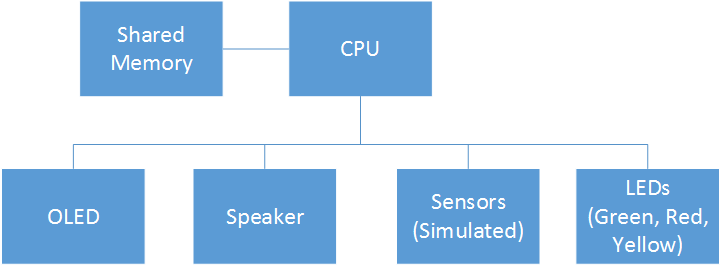
\includegraphics[width=\textwidth]{../design/Functional_decomposition}
      \caption{Functional Decomposition}
      \label{fig:func}
    \end{figure}

    \subsubsection{System Architecture}
    Next, the system architecture was developed (Figure~\ref{fig:arch}). At a high
    level the system works on two main concepts, the scheduler and tasks. Tasks
    embody some sort of work being done, and the scheduler is in charge of
    determining the speed and order in which the tasks execute. The system has
    several tasks, each with their own specific job. For modularity reasons, each
    task should have the same public interface and the scheduler should be able to
    run each task regardless of that specific tasks job or implementation. Thus
    the task concept is abstracted into a Task Control Block (TCB), and the
    scheduler maintains a queue of TCBs to run. The TCB abstraction is shown in
    Figure~\ref{fig:arch} using inheritance, and the fact that the scheduler has a
    queue of TCBs is shown with composition. The core functionality of the system
    was divided into the following eight main tasks:

    \paragraph{Initialization Task} This task Initializes data structures and does
    system startup-related jobs. This task is not actually scheduled to run, it
    only executes a single time at system startup.

    \paragraph{Measure Task} The measurement task is in charge of interacting with
    the blood pressure, temperature, and pulse sensors. Each of these is
    simulated. The blood pressure and temperature are simulated in the CPU. The
    task will measure the pulse rate by parsing an externally generated square wave
    of varying frequency; the pulse rate being proportional to the frequency.

    \paragraph{Compute Task} Compute takes the simulated raw data and converts it to the
    correct units of measurement. Raw temperature data to Celsius, blood pressure
    to mm Hg, and pulse rate to BPM.

    \paragraph{Keypad Monitor} Keypad will check the keypad for user input. It
    should provide the user with four keys: two for scrolling, one for selection,
    and one to go back.

    \paragraph{Display Task} The display task will show a user interface on the
    Stellaris OLED. The user will interact with the display using a keypad. Under
    normal operation, a menu will be displayed asking users which measurement they
    would like to see. If the user presses back while in this menu, they enter
    annunciate mode which displays all the measurements currently in warning or
    alarm state.

    \paragraph{Warning/Alarm Task} Under normal operation, this task will light a
    green LED signifying that everything is OK. If one of the measurements enters
    a warning state, the task will flash a red LED at a rate specific to the
    warning for that measurement. If there is an alarm state, it sound the alarm
    by driving the speaker. At any time if the battery goes too low, the yellow
    LED will illuminate.

    \paragraph{Remote Communication Task} This task is in charge of sending data to
    a remote terminal. If any of the states are in a warning or alarm condition,
    this task will transmit the (corrected) data to the remote terminal.

    \paragraph{Status Task} Status receives information about the battery on the
    system and updates it's current data accordingly.
    \\\\
    Each of these tasks interact using the shared data shown in Figure~\ref{fig:arch}. 

    \begin{figure}[h]
      \centering
      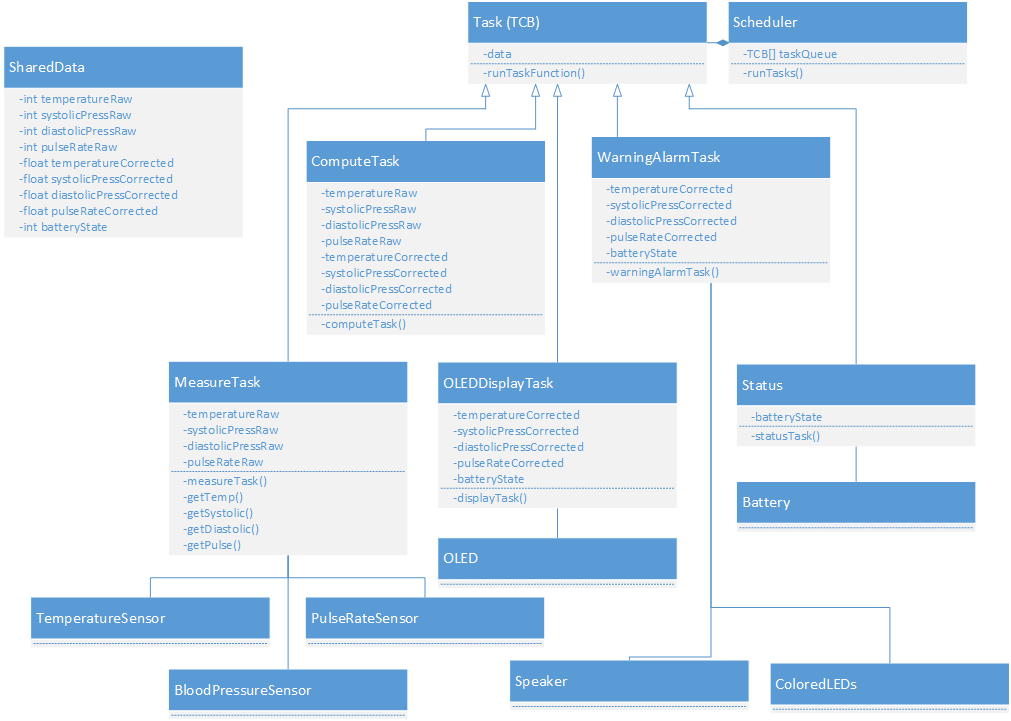
\includegraphics[width=\textwidth]{../design/System_Architecture}
      \caption{System Architecture Diagram}
      \label{fig:arch}
    \end{figure}

    \subsubsection{High-level Implementation in C}
    After developing the system architecture, the design needed to be translated into the C programming language. The design manifested in a multi-file program consisting of the following source files:
    \begin{itemize}
      \item \textbf{globals.c/globals.h} - Used to define the Shared Data used among the tasks
      \item \textbf{schedule.c/schedule.h} - Defines the scheduler interface and it's implementation, as well as the TCB structure
      \item \textbf{timebase.h} - Defines the timebase used for the scheduler and tasks
      \item \textbf{task.h} - Defines the TCB interface for a task
    \end{itemize}
    Each task also has it's corresponding ``.c'' and ``.h'' file (for example, measure.c and measure.h).

    The TCB structure that the scheduler uses must work for all tasks, and must not
    contain any task-specific information. Instead, the TCB consists of only a void pointer to the tasks data, and a pointer to a function that returns void and takes a void pointer, as follows:
    \begin{lstlisting}
    struct TCB {
      void *taskDataPtr;
      void (*taskRunFn)(void *);
    }
    \end{lstlisting}
    Leaving out the type information allows the scheduler to pass the task's data
    (*taskDataPtr) into the task's run function completely unaware of the kind of
    data the task uses or how the task works.

    For increased modularity, the data structure used by each task was not put in
    the task's header file. Instead, the structure was declared within the task
    implementation file, and instantiated using a task initialization function. In
    the header file, a void pointer pointing to the initialized structure is
    exposed with global scope, as well as the task's run and initialization functions.

    \subsubsection{Task Implementation}

%implementation details here. Tasks, scheduler, etc. Control diagram goes here,
%activity diagram, etc.

    The primary task of this project is to implement C code for a medical device on
    the Stellaris EKI-LM3S8962 and its ARM Coretex A3 processor. The project was
    started by creating a main file that initializes the variables used in each
    task and starts the hardware timer then runs into an infinite while loop. Inside the while loop a run method
    is called. The run method is part of the scheduler. The run method has a runTask flag which determines whether or not anything should actually be run this call. The flag is set to true by the hardware timer's interrupt handler. Once the runTask flag is true the run method will keep track of
    whether the device is on a minor cycle or a major cycle and run the preform
    task method of each task. The runTask flag is then set to false so that the tasks will not be executed again until the hardware interrupt has again been triggered. The tasks included in this project are Compute,
    Measure, Warning, keyPad, oledDisplay, Serial, and status. Each task has a public interface of
    2 void pointers. One that when initialized by the main method will point to the
    preform task function, and another that, when initialized, points to a struct
    containing pointers to the data required by that task. Each task has a task
    control block(TCB) in the scheduler. This TCB contains pointers to the
    preform task function and the data for the task and also has fields for pointers to a next TCB and previous TCB. The TCB is used by the
    scheduler to run the task. The scheduler contains a doubly linked list of TCB objects that uses the TCB next and previous elements to point to the next and previous tasks in the task queue. In this case there are 7 tasks but not always 7 tasks in the list of tasks to run. The compute task is only to be run after the measure task, and the serial task only needs to be run at certain times. When a task is not being used it's TCB is not included in the linked list of tasks. Therefore and updateQueue method was created. This method checks flags set within the tasks that are running and determines if a task that isnt in the list needs to be added, or if a task that is in the list needs to be removed. The scheduler's run task contains a loop that runs
    through the linked list of TCBs and runs the function pointed to by the TCB with the
    argument of the data pointer stored in the TCB until the null value pointed to by the last element in the list is reached. After running all  tasks the
    runTask flag is set to false again. The hardware timer will count up until it reaches the number of ms that corresponds to a minor cycle then trigger a hardware interrupt. The interrupt handler sets the runTask flag back to true and the task linked list will be updated, traversed and run again.
    
    control flow is shown in Figure~\ref{fig:Control}. 

    \begin{figure}[h]
      \centering
      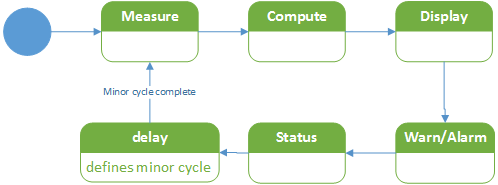
\includegraphics[width=0.8\textwidth]{../design/Control_state_diagram.png}
      \caption{Control Flow Diagram}
      \label{fig:Control}
    \end{figure}

    Each task has its own unique purpose in the system, and each uses a different
    part of the global data.

    \paragraph{Measure Task}
    The Measure task (Figure~\ref{fig:measureActivity} in the
    appendix), deals only with the raw data from the instruments. This task is
    meant to act in place of the instruments that are unavailable. The task only
    runs if the scheduler has set the global value is Major Cycle to 1. On a major
    cycle the measure function either increments the data of each measurement by 1
    or 2 or decrements the data by 1 or 2. In the newly improved design a heart rate monitor has been added. The heart rate monitor uses an interrupt handler to count the number of rising edges on an input in a 2 Major cycle period. The number is then used to calculate the heart rate the sensor is receiving. Additionally the measure task adds the compute task to the task queue after it has run.

    \paragraph{Compute Task}
    The compute task is very simple. This task will only run after it has been placed into the task queue by the measure task and it will remove itself from the queue after running. It takes the raw data that has been set by the measure task, multiplies
    by a constant and adds a constant to each piece of raw data to get the
    corrected data. The compute task then puts the values for the corrected data in
    memory at the location of the global data pointer. Compute uses every data
    value except the battery and keypad data. A diagram of the Compute activity is shown in the appendix in Figure~\ref{fig:computeActivity}.

    \paragraph{Warning Task}
    After compute, the warning task begins checking for warning or alarm states. The
    warning task only deals with the corrected data from compute and the battery
    state. This task also must deal with the input and output signals used to
    display warning and sound an alarm. Unlike the other tasks, this task has more
    to its initialization than just initializing the data. In addition to setting
    up the pointers to the global data, during initialization, the task also
    enables peripheral banks C, F, and G. These are enabled using the
    SysCtlPeripheralEnable library call. Additionally the task set up pins C 5, 6,
    and 7 as outputs, and pins F 0 and G 1 as PWM outputs. Additionally the PWM outputs are set to use a 65 Hz clock to play
    a sound at this frequency whenever enabled. The activity diagram is shown in
    Figure~\ref{fig:warningActivity} in the appendix. There are 3 subsystems in the
    warning task. These subsystems each handle a different part of user
    notification. The first subsystem deals with the alarm. The subsystem checks to
    see if the systolic blood pressure data is out of range by more than 20\%. If the value is out of that range then the PWM output is enabled
    using PWMGenEnable and pulsed with a 2 second period. If the values fall back within the acceptable range, or the
    user hits the acknowledge button, then the PWM is disabled with PWMGenDisable
    and the sound stops. The acknowledge button is sensed in the keyPad task and a global data value global.alarmAcknowledge is set. When the alarmAcknowledge field is set to 1 the alarm will go to its resting state. The next subsystem checks the corrected data for being 5\%
    out of range of the accepted values. If any value is more than 5\% out of its
    range then a warning will be displayed on the red led connected to pin C 5
    using the GPIOPinWrite function. Depending on the value that is out of range
    the period the led flashes at will vary. In addition to the led flashing the warning will also tell the scheduler to add the serialCommunication task to the task list. The final subsystem is the battery
    check. This system checks if there is more than 30\% of battery left on the
    device. This is taken from the battery state data field. If there is less than
    20\% battery left then a yellow led connected to pin C7 is illuminated, if
    there is more then 20\% battery, and the device is not in a warning or alarm
    state then the green led on pin C 6 is illuminated. 
    
    
	\paragraph{Keypad Task}
    The keyPad task uses the gpio libraries to set up 5 inputs. 1 input is pin E 0 and is used as the alarm acknowledge button. The other 4 pins are inputs on pins D 4, D 5, D 6, and D 7, and are used to detect button presses on the external keypad. The keypad works by connecting 2 of the outputs from the keypad together. There are 4 row outputs and 4 column outputs for a total of 16 possible combinations. The design was simplified by only using 1 column of 4 buttons. By doing this, the column keyPad wire can be supplied with a constant 5V from the Stellaris board, then each of the 4 row lines can be connected to a GPIO input. when a button in the live column is pushed the 5V column line is connected to 1 of the GPIO pins which lets the keyPad task know which button was pushed. Every time the keyPad task is run the GPIO will tell the task what buttons are pressed. 2 of the buttons correspond to up and down for scroll in the menu, 1 button corresponds to select in the menu, and 1 button changes the mode between menu and annunciation. The data that the buttons manipulate are the global keyPad data parts which are global.select, global.scroll, and global.mode. Additionaly the input on pin E 0 manipulates the global.alarmAcknowledge signal. The activity diagram for this task is shown in the appendix in Figure~\ref{fig:keyPadActivity}.
    \paragraph{Display Task}
    To show a user their current medical measurements, the system also has an
    oledDisplay task. This task uses the corrected data from measurements, the
    battery state, and the keyPad data. The display task has an activity diagram shown in
    Figure~\ref{fig:displayActivity} in the appendix. This task uses the usnprintf()
    function in C to convert the data types that the corrected data is stored in,
    and properly format these data values into a string which is stored in a
    buffer. The string contained in the buffer is then printed to the OLED screen
    using the driver library rit128x96x4 functions. The display has 2 modes. The mode that the screen currently displays is determined by the global.mode data which is set in the keyPad task. When mode is 0 this is the menu mode. This mode displays each of the 4 measurement types, temperature, blood pressure, pulse rate, and battery without the data for each. The task then takes the global.scroll data from keyPad and displays a cursor next to the measurement that scroll is currently at, 0 corresponding to temperature, 1 to blood pressure, and so on. If the global.select is set to 1 in keyPad then the currently scrolled to measurement is selected and the screen will change to showing only that measurement and its data. When global.mode is equal to 0 the annunciation screen will instead be displayed. This screen shows each measurement followed by its data.
    
	\paragraph{Serial Task}
    The serial task is only run when a warning occurs. The warning causes the TCB for the serial task to be added to the TCB schedule linked list. When the serial task is run the first time it will initialize a UART connection using UARTConfigSet and UARTEnable driver functions to enable the UART that communicates to an FTDI chip on the Stellaris board. The FTDI chip then converts the UART to a virtual serial port over the usb cable to the PC. After the UART is initialized on the first run and in all subsequent runs of the serial task, all the measurements and their data are formatted and printed into 1 buffer using the usnprintf function. A loop then itterates through the buffer writing each character in the buffer to the UART. An activity diagram showing the serial task is located in the appendix as Figure~\ref{fig:serialActivity}.
    
    \paragraph{Status Task}
    The last task is the status task. This task only deals with one piece of data
    which is the battery state data. The only thing the status task does is that on
    a major cycle, it decrements the battery state by 1. This is shown in the
    activity diagram in Figure~\ref{fig:statusActivity} in the appendix.

    \section{Presentation, Discussion, and Analysis of the Results}

    \subsection{Results} Patrick

    The project was completed and demonstrated on February 13, 2014.

    Demonstration of the system to the interested parties showed that the
    system met the majority of the requirements initially presented at the onset of the lab
    project.  Testing of the system prior to demonstration also verified that
    the system met the specifications listed in Section~\ref{sec:designSpec}.

    During the demonstration, all tasks worked as designed and expected with the exception of

    During the actual coding and implementation of the design, remarks were
    made several times about the ease of execution during that phase of the
    project. After the initial high level Design phase, very few changes were
    made, or required, to the functional design or system architecture.

    Using an oscilloscope, the run times of each task were empirically
    determined. The results are given in Table~\ref{tab:taskRuntimes}.

    \begin{table}[h]
      \centering
      \begin{tabular}{|l|r|} 
	\hline
	Task & Runtime ($\mu$s) \\ \hline
	Measure & 23.4 \\ \hline
	Compute & 55.4 \\ \hline
	Display & 22900.0 \\ \hline
	Warning & 27.4 \\ \hline
	Status & 5.6 \\ \hline
      \end{tabular}
      \caption{Empirically determined task runtimes}
      \label{tab:taskRuntimes}
    \end{table}

    \textbf{Answers to the last three questions in the list of items to include
    in the project report:}
    \emph{You don't find the stealth submarine. That's why they are so expensive; at that cost, you take great pains to never lose one.\\  A helium balloon always rises. It just rises upside-down. \\ If you really managed to lose the stealth submersible, you first have to tell the government, which will deny it has any stealth submersibles, then you have to comb the seven seas until your comb hits the sub.}

    \subsection{Discussion of Results}
    The ease of change in the code is the result of a large amount of time spent on
    design. The design makes it easy to configure flash times, add new tasks, and
    to reason about tasks independently of the whole system. The solid high-level
    architectural design led to ease of implementation and change.

    In terms of performance, the run times of each task appear to correspond with
    the number of instructions required for each task. Given the speed of the CPU,
    8 MHz, we can calculate an estimated number of instructions for each task.
    This is given in Table~\ref{tab:instr}.
    \begin{table}[h]
      \centering
      \begin{tabular}{|l|r|} 
	\hline
	Task & Instructions \\ \hline
	Measure & 187 \\ \hline
	Compute & 443 \\ \hline
	Display & 183,200 \\ \hline
	Warning & 219 \\ \hline
	Status & 45 \\ \hline
      \end{tabular}
      \caption{Estimated instructions per task, rounded to the nearest instruction}
      \label{tab:instr}
    \end{table}
    The majority of the cycles are likely spent waiting for memory. For example,
    the status task only has two comparisons and an arithmetic operation, but has
    to reference the data in global memory. The exception here is the display
    task, which was about three orders of magnitude more instructions than the
    other tasks. This was due to the sprintf() library call, included in the
    standard C library. While this could have been optimized, it was found that
    with a minor cycle delay of 250 ms, the display delay of 22.9 ms was not
    significant.


    \subsection{Analysis of Any Errors}

    - BPM Range error
    - Serial error
    
    There were two errors found in the final project.  First, the pulse rate
    range is not exactly as specified.  Second, it was found that the serial
    communications task did not produce the correct values.

    The specified corrected pulse rate was to be between 10 BPM and 200 BPM.
    For simplicity, the raw pulse rate was implemented as a 1-1 mapping from
    frequency to raw pulse rate.  For example, a 1 Hz frequency would produce a
    value of 1 for raw pulse rate, and a 15 Hz signal would produce a value of
    15 for raw pulse rate.  This caused two issues.  When the Input frequency
    is 1, the measured BPM (using the specified raw to correct conversion) is
    $8 + 3\cdot(1) = 11 BPM$.  This is larger than the specified 10 BPM
    minimum.  Also, when the input frequency is 64 Hz, a corrected value of 
    $8 + 3\cdot(64) = 200 BPM$ is expected.  However, as the frequency
    increased, the overhead of the other running tasks became significant.
    As a result, more rising edges could fit in our measurement interval
    than we expected.  This resulted in a maximum BPM of roughly 206 BPM.

    There was also an error in the Serial communication protocol in which the
    usnprintf command used to format the data was causing a runtime error when
    printing formatted data to a buffer.  Rather than printing the actual
    corrected values to the buffer (to be sent to the remote terminal), it
    seemed the command was printing addresses.  It was believed this was
    caused by an error with the CircularBuffer implementation, though no
    other tasks had issues with it (and extensive tests validated the 
    CircularBuffer).  

    \subsection{Analysis of Implementation Issues and Workarounds}

%State any problems you encountered while working on the project. If your
%project did not work or worked only partially, provide an analysis of why and
%what efforts were made to identify the root cause of any problems. \\

%Some points to bring up: did not enable the GPIO bank (caused OLED display to
%not work), could not get switch to work (solved by understanding that switch
%required pull up). P or J can talk about design solutions that did not work.
%On the whole, had problems with going too deep, too quickly.

  The medical instrument design in this project was completed and tested
    successfully to meet almost all the requirements, the designers did face a few difficulties in designing the device, however, because this design was additional functionality added to a previous projects design, many of the errors previously encountered were easily avoided due to experience of the students, and already completed coding work.
    
    
    Many of the challenges the designers of this project faced were in the keypad input and the data output. The keypad input posed a difficult hardware challenge as there are 16 input keys on the keypad but only 8 connections for the microprocessor to connect to the keypad. This means that to identify a single key press 4 connections must be set as outputs and 4 as inputs. The inputs can then be scanned as the outputs are set 1 at a time to find which key is pressed. Instead of implementing this design, the students instead opted to use only 4 buttons on the keypad. This allowed the strobe design to be ignored. Instead 1 row of keys was activated all the time and that row was scanned for button presses.
    
    In addition to keypad input, there was also difficulty in implementing data formatting functions. After adding a hardware delay, IAR workbench no longer allows the use of sprintf which had previously been used to print and format data. The usnprintf command was instead used to format and print data to a buffer, however, the students found that usnprintf does not have the ability to print floating point data. This issue was resolved by changing measurements that were previously printed as floats to be printed as integers. Usnprintf also caused issues when printing certain data for the serial task. In this case the usnprintf was causing a runtime error and freezing the operation of our device. This issue remained unresolved. 
    
    
    
    
    All problems but one were solved before demonstrating the product to the interested
    parties. The final project still contained the serial error previously mentioned.
    
    \section{Test Plan} 

    To ensure that this project meets the specifications listed in 
    section~\ref{sec:designSpec}, the following parts of the system must be 
    tested: 

    \begin{itemize}
      \item Vitals are measured and updated
      \item System properly displays corrected measurements and units properly
      \item System enters, indicates, and exits the proper warning state for
	blood pressure, temperature, pulse, and battery
      \item System enters and exits the alarm state correctly
      \item Alarm is silenced upon button push
      \item Alarm recommences sound after silencing if system remains in alarm
	state longer than silence period
    \end{itemize}

    Additional tests to determine the runtime of each specific task are also
    required.

    The inclusion of additional specifications for Phase II of the project
    requires additonal tests to ensure the system meets the customer
    requirements.

    \textbf{Phase II Tests:}
    \begin{itemize}
      \item Scheduler loops through linked list properly
      \item Scheduler adds and removes from the linked list the following tasks
	correctly:
	\begin{itemize}
	  \item Compute task added by measure task
	  \item Serial communication task added by annunciation task
	  \item Compute task removed by itself
	  \item Serial communication task removed by itself
	\end{itemize}
      \item Warning task alarm meets the following two requirements
	\begin{enumerate}
	  \item Has one (1) second tones; a total period of 2 seconds
	  \item Activates only when systoic pressure is greater than 20\% above
	    normal
	  \item Has an auditory deactivation or ``sleep'' period of 5
	    measurement cycles
	\end{enumerate}
	\item Serial task displays the temperature, blood pressure, pulse rate,
	  and battery status as listed in Section~\ref{sec:designSpec}
	\item Keypad task captures user inputs, sets the appropriate inputs,
	  and causes the assocated changes in system state
	\item Hardware timer updates the system's mnor cycle counter
    \end{itemize}

    More detailed explanation of the tests performed is provided in the
    following sections.
    
    \subsection{Test Specification} 

%    Annotated description of what is to be tested and the test limits. This
%    specification quantifies inputs, outputs, and constraints on the system.
%    That is, it provides specific values for each. 
%
%    Note, this does not specify test implementation...this is what to do, not
%    how to do it.

    \subsubsection{Scheduler}
    The scheduler needs to be shown to correctly schedule and dispatch tasks.
    This means that task should execute in the right order, and at the right
    time. Given a minor cycle of 50 ms, every task should run roughly once
    every 50 ms.   Also, the scheduler needs to successfully add and remove
    tasks from the queue dynamically.  Specifically, the Measure Task
    should be able to tell the scheduler to add the Compute Task and the
    Warning/Alarm Task should be able to schedule the Serial Task.  Both
    Compute and Serial should be able to be removed from the schedule.

    \subsubsection{Measure Task}
    For this design, the temperature and blood pressure values were simulated
    on the CPU.  The pulse rate was simulated using an externally generated
    square wave of varying frequency.  
    \begin{itemize}
      \item \textbf{Temperature} The temperature should increase by two every
	even major cycle (5 seconds) and decrease by one ever odd major cycle
	until it exceeds 50, at which point the process should reverse
	(decrease by two every even major cycle and increase by one every odd
	major cycle), until it dips below 15, and the whole process should be
	started over again. 
      \item \textbf{Pulse}  The pulse rate should match one-to-one with the
    frequency of the input signal.  For example, a 15 Hz signal should produce
    a raw pulse rate of 15.
      \item \textbf{Systolic Pressure} The systolic pressure should increase by
	three every even major cycle and decreases by one every odd major
	cycle. If it exceeds 100, it should reset to an initial value.
      \item \textbf{Diastolic Pressure} The diastolic pressure should decrease
	by two on even major cycles and decrease by one on odd major cycles,
	until it drops below 40, when it should restart the process.
    \end{itemize}

    The Measurement Task should also successfully add the Compute Task to the 
    schedule queue.

    \subsubsection{Compute Task}
    The compute task should be verified to convert raw simulated sensor data
    according to the following formulas.
    \begin{itemize}
      \item $CorrectedTemperature = 5 + 0.75 * RawTemperature$
      \item $CorrectedSystolicPressure = 9 + 2 * RawSystolicPressure$
      \item $CorrectedDiastolicPressure = 6 + 1.5 * RawTemperature$
      \item $CorrectedPulseRate = 8 + 3 * RawTemperature$
    \end{itemize}

    The compute task should also successfully remove itself from the schedule
    queue.

    \subsubsection{Keypad Task} 
    The keypad should be tested to successfully
    capture user input.  When the select button is pressed, the measurement
    selection value should reflect the selected measurement.  When the up
    scroll button is pressed, the scroll value should be incremented, and when
    the down scroll button is pressed, the scroll value should be decremented.  
    If the alarm acknowledge button is pressed, this should be reflected in 
    the alarmAcknowledge global value.

    \subsubsection{Display Task}
    On load, the display task should present the user with an option to select
    the desired measurement.  If the back button is pressed, the annunciation
    screen should be displayed, showing the measurements in warning or alarm
    state.  

    \subsubsection{Warning/Alarm Task} 
    The warning/alarm system needs to be tested to do several things. When in a
    warning state, it should flash the red LED at the rate appropriate for the
    warning. When the battery is low, it should illuminate the yellow LED. If the
    system is in an alarm state, it should sound the speaker alarm. The following
    ranges in Table~\ref{tab:ranges} are calculated from the specified minimum and
    maximums found in Table~\ref{tab:sensorDefs} on page \pageref{tab:sensorDefs}.
    \begin{table}[h]
      \centering
      \begin{tabular}{lcr} 
	\toprule
	Data & Warning Range & Alarm Range \\
	\midrule
	Temperature & 34.3 - 39.7 C & 32.5 - 41.6 C\\
	Systolic Pressure & $>$ 84 mmHg & $>$ 88 mmHg\\
	Diastolic Pressure & $>$ 126 mmHg & $>$ 132 mmHg\\
	Pulse & 57 - 63 BPM & 54 - 110 BPM \\
	\bottomrule
      \end{tabular}
      \caption{Initial values and warning/alarm states}
      \label{tab:ranges}
    \end{table}

    This task should also add the Serial task if any of the measurements are in
    a warning or alarm condition.

    \subsubsection{Serial Task}
    If any of the measurements are in warning or alarm state, this task should
    send this data serially to a remote terminal.  The task should send all the
    data (not just the data in warning or alarm state).  It should be printed in 
    the following format:

    % Oddly, the following can't be indented or weird stuff will happen
\begin{lstlisting}
1. Temperature              0 C
2. Systolic Blood Pressure  0 mm Hg
3. Diastolic Blood Pressure 0 mm Hg
4. Pulse Rate               0 BPM
5. Battery                  0 % 
\end{lstlisting}

    \subsubsection{Status Task}
    Since the initial design does not use a battery, the status task simulates the
    battery state using the CPU. For now, it simply decrements the state of the
    battery. The test should show that the battery state is decremented by one
    every major cycle.

    \subsection{Test Cases}

    The students begin testing by examining if the alarm sounds at the proper time.
    This is initially tested by disabling the functions that simulate measurements
    being made on each of the data measurements, and setting their initial values
    to be either within the alarm range or outside of the alarm range. The warning
    states were also initially tested this way. The initial values for raw data
    given in Table~\ref{tab:sensorDefs} on page \pageref{tab:sensorDefs} were used
    to test the normal state of the machine because each falls within the
    acceptable range of measurements for corrected data (also given in
    Table~\ref{tab:sensorDefs}) that does not require a warning.
    Using these initial values, the code was programmed onto the Stellaris board.
    Correct operation was verified by the alarm not sounding, and the red led being
    off, indicating that no warning state was in effect. In addition the green led
    was on indicating a normal state. Next the students varied one parameter at a
    time to be outside of the acceptable range by more than 10\%. Starting with the
    temperature being set to an initial raw value of 50, the alarm was verified by
    hearing the aural annunciation coming from the system. In addition, the
    temperature warning stat was also in effect. This means that the green led was
    off and the red led was blinking. To verify correct operation we needed to make
    sure the led was blinking with a period of 1 second. The correct flashing
    pattern was verified by counting the number of times the led flashed in 6
    seconds. In this case, for temperature, the led flashed 6 times in 6 seconds
    indicating a 1 second period, and correct operation. After this test, the
    temperature value was returned to 42 and the Pulse was instead set to 45. The
    same methods were used to verify that the alarm and warning states for pulse
    rate were working correctly, but this time the warning led turned on 3 times in
    6 seconds indicating a 2 second period which is the intended period of
    flashing. The pulse rate was then returned to 25 and each pressure reading was
    checked for correct operation individually by being set to an initial raw value
    of 100. Once again, the green led started off because the system was not in a
    normal state. The alarm was sounding due to the extremely high blood pressure
    measurements, and the red warning led flashed 12 times in 6 seconds indicating
    the correct period of .5 seconds for a blood pressure warning. In addition to
    testing the validity of each warning state and alarm state, the acknowledgement
    of the alarm was also tested during each of these tests. This was tested by
    hitting the acknowledge button once during each measurements test. During each
    test, hitting the acknowledge button turned the alarm sound off for a short
    time, as intended. 


    Next the measurement simulation functions were tested. This was done by
    re-enabling each one that had been disabled from the previous test one at a
    time. The initial raw values were again set to the values in Figure 5. When
    each measurement was re-enabled, the students could watch the temperature change
    at each major cycle using the OLED display. Since the OLED display indicated
    that the corrected temperature went up .75 degrees on a major cycle then down
    1.5 degrees on the next, the temperature measurement was working as intended.
    This situation also gave the students an opportunity to verify that the warning
    and alarm states initiated as the temperature fell out of the acceptable range.
    The Led began flashing with a 1 second period after a few major cycles, then
    the alarm began sounding, indicating correct operation. Since temperature was
    working correctly, the temperature measurement function was once again disabled
    and each blood pressure measurement was
    re-enabled individually for testing. The Systolic pressure began by rising 4 mm
    Hg on a major cycle then falling 2 mm Hg on the next, and the Diastolic
    pressure by rising 3 on a Major cycle and falling 1.5 on the next, this was
    consistent with the design. The warning and alarm states were activated as each
    passed its threshold and the red led was blinking with a period of .5 seconds.
    The warning led was also tested in the case that all warning states were
    active. To do this all initial values were set to 100. In this case, as
    designed by the students, the red warning led indicated the fastest blinking
    warning with a .5 second period. 
    
    In this device, a new pulse rate monitor device was added. To test the pulse rate monitor  the monitor input was connected to a function generator generating square waves. As the square wave frequency was increased the pulse rate value was expected to increase. This was verified to be working correctly. As the pulse rate passed through the warning zones the design for pulse rate warnings was also verified to be working correctly.
    
    Additionaly, the improved medical device now has a menu that is displayed on the oled display and navigated using the testbench keypad. The design operating these functions was tested by navigating to each part of the menu using the keys on the keypad and visually verifying that each part of the menu displayed the correct data. Each menu, annunciation, main menu, and each measurements selection mode, was visually verified to be working as intended. The keypad functionality was verified as each button was used to navigate through the menu.
    
    The newly added serial communication was then tested using the hyperterm program on the lab station PC. The serial connection was established over a virtual COM port on the usb connection from the PC to the Stellaris board. The program had the intended functionality of displaying each of the measurements, and its current data on the serial port whenever the alarm state was entered. The functionality could be verified by watching the hyperterm screen to see if the data displayed when a warning state occured. The data on hyperterm could then be compared to the oled display data to verify its accuracy. 
    
    

    The final bit of testing preformed on the system was timing each task within
    the system. This was done by adding a general purpose output pin in the
    scheduler code. This output was set high right before the execution of a task,
    and set low immediately after the execution of the task. An oscilloscope was
    then attached to this output pin and set to trigger on a positive edge. The
    cursors were then used to measure the amount of time the signal was high in
    each cycle.


    \section{Summary and Conclusion}

    \subsection{Final Summary} The students began creating their medical instrument
    through a rigorous design process at different levels of detail. The students
    then continued work by implementing their design in C code for the ARM Cortex
    A3 microprocessor. Next the code was tested and debugged using the IAR
    workbench debugging tool, as well as visual queues programmed into the design.
    Finally, after verifying that the system worked as specified, it was presented
    to the instructor.

    \subsection{Project Conclusions} This project contained 3 major phases, the
    design, implementation, and testing steps. The students were immediately
    introduced to using the unified modeling language(UML) to design embedded
    systems. This is the first time many students will have used UML for system
    design which caused some confusion and difficulty. In the end through the use
    of the UML guidelines for design, the students were able to implement their
    system in code for the Texas Instruments Stellaris EKI-LM3S8962 much more
    quickly and with far fewer errors than if they had spent less time in the
    design phase of this project. 

    Effective design tools allowed the students to quickly implement their embedded
    system in C code for an ARM Cortex A3 processor, and move onto the testing
    phase of the project quickly. Unfortunately, while testing the students
    encountered a number of problems in using the PWM and general purpose input and
    output signals. After consulting the documentation for the Stellaris kit and
    solving their input/output problems, they began testing their design using
    visual and audio queues, the IAR embedded workbench debugger, and a few
    specifically programmed debug features. After the results of the testing
    verified the design to be working correctly, the students proceeded to present
    their medical instrument to their instructor.

    \pagebreak
    \appendix

    \section{Breakdown of Lab Person-hours (Estimated)}

    \begin{tabular}{|l|*{4}{r|}}
      \hline
      Person & Design Hrs & Code Hrs & Test/Debug Hrs & Documentation Hrs \\ \hline
      Patrick & 20 & 10 & 10 & 12+  \\ \hline
      Jonathan & 15 & 5 & 4 & 8  \\ \hline
    \end{tabular}

    ~\\

    By initializing/signing above, I attest that I did in fact work the
    estimated number of hours stated. I also attest, under penalty of shame,
    that the work produced during the lab and contained herein is actually my
    own (as far as I know to be true). If special considerations or
    dispensations are due others or myself, I have indicated them below.

    \pagebreak

    \section{Activity Diagrams}

    \begin{figure}
      \centering
      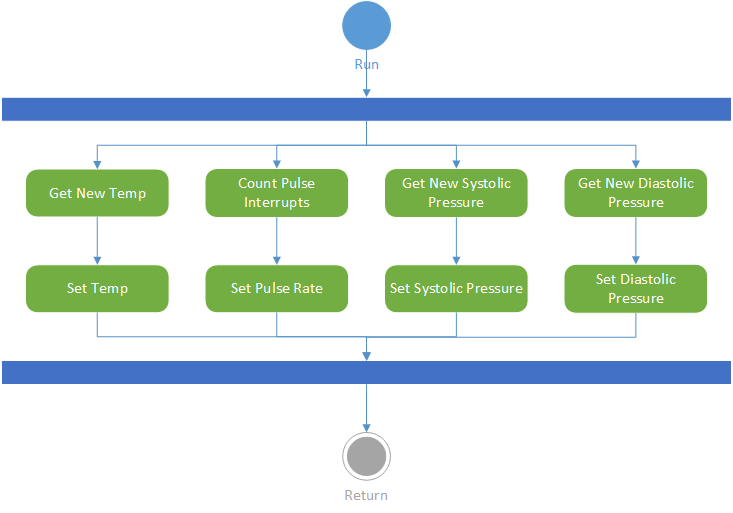
\includegraphics[width=\textwidth]{../design/measure_activity.png}
      \caption{Measure Activity Diagram}
      \label{fig:measureActivity}
    \end{figure}

    \begin{figure}
      \centering
      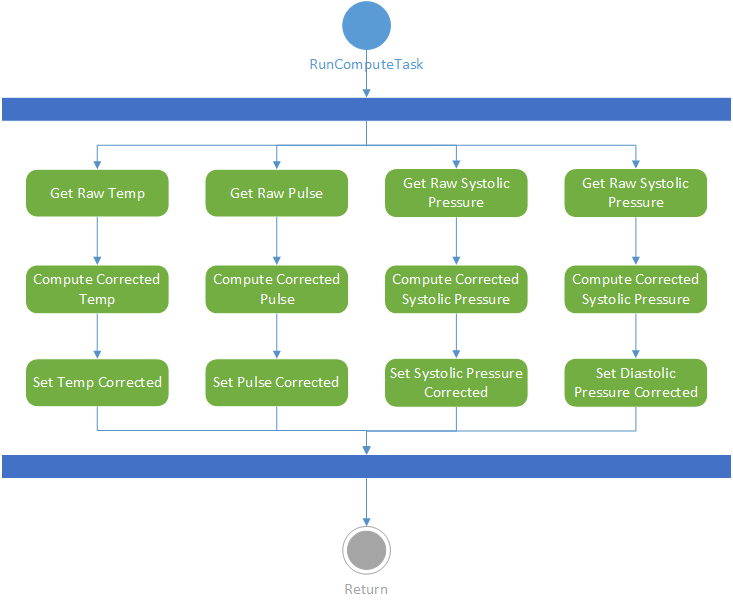
\includegraphics[width=\textwidth]{../design/compute_activity.png}
      \caption{Compute Activity Diagram}
      \label{fig:computeActivity}
    \end{figure}

    \begin{figure}
      \centering
      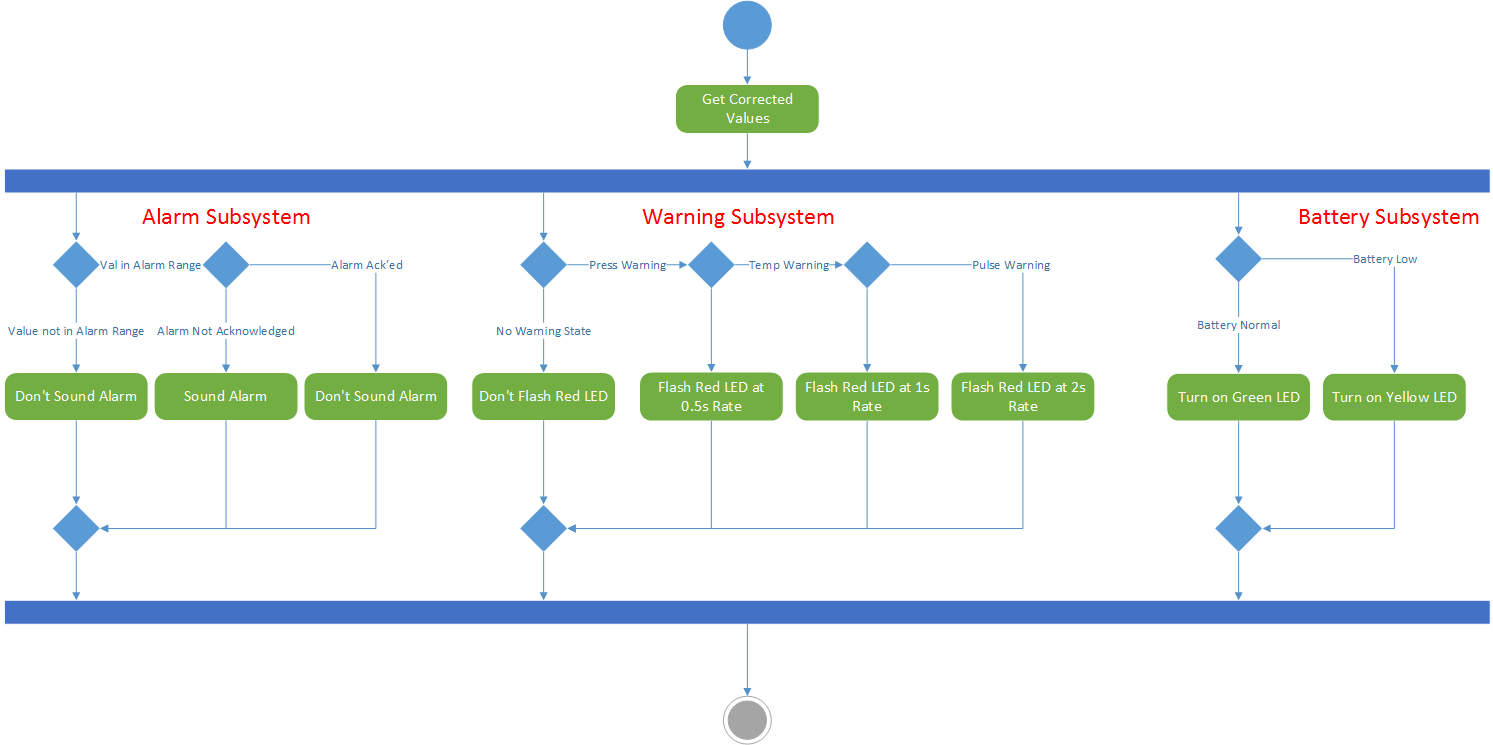
\includegraphics[width=\textwidth]{../design/warning_activity.png}
      \caption{Warning Activity Diagram}
      \label{fig:warningActivity}
    \end{figure}

    \begin{figure}
      \centering
      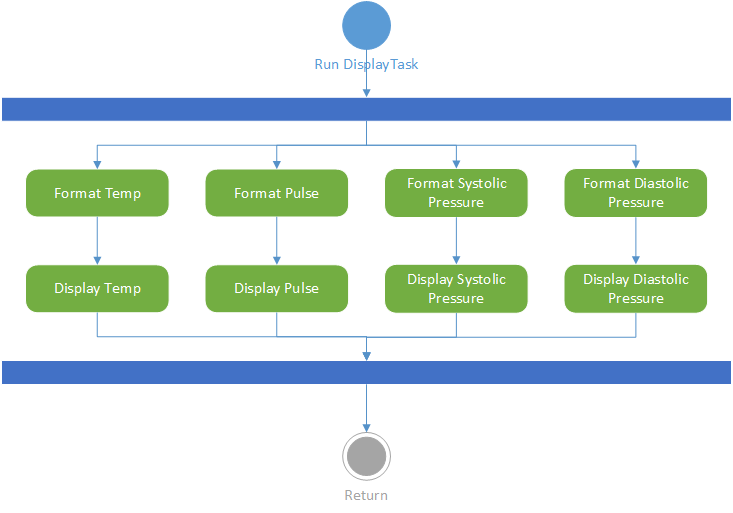
\includegraphics[width=\textwidth]{../design/display_activity.png}
      \caption{Display Activity Diagram}
      \label{fig:displayActivity}
    \end{figure}

    \begin{figure}
      \centering
      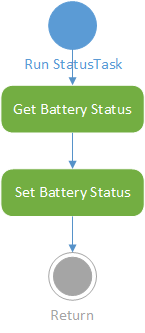
\includegraphics[width=0.2\textwidth]{../design/Status_activity.png}
      \caption{Status Activity Diagram}
      \label{fig:statusActivity}
    \end{figure}

    \pagebreak

    \section{Source Code}

    Source code for this project is provided below.

    \subsection{Main Function}
    \lstinputlisting{../code/main.c}

    \subsection{Global Data}
    \lstinputlisting{../code/globals.h}
    \lstinputlisting{../code/globals.c}

    \subsection{Timebase}
    \lstinputlisting{../code/timebase.h}

    \subsection{Scheduler}
    \lstinputlisting{../code/schedule.h}
    \lstinputlisting{../code/schedule.c}

    \subsection{Tasks}
    \subsubsection{Measure Task}
    \lstinputlisting{../code/measure.h}
    \lstinputlisting{../code/measure.c}

    \subsubsection{Compute Task}
    \lstinputlisting{../code/compute.h}
    \lstinputlisting{../code/compute.c}

    \subsubsection{Display Task}
    \lstinputlisting{../code/display.h}
    \lstinputlisting{../code/display.c}

    \subsubsection{Warning/Alarm Task}
    \lstinputlisting{../code/warning.h}
    \lstinputlisting{../code/warning.c}

    \subsubsection{Status}
    \lstinputlisting{../code/status.h}
    \lstinputlisting{../code/status.c}

    \end{document}
